% *********************************************************************
% © 2021–2026 Jeremy Sylvestre
%
% Permission is granted to copy, distribute and/or modify this document
% under the terms of the GNU Free Documentation License, Version 1.3 or
% any later version published by the Free Software Foundation; with no
% Invariant Sections, no Front-Cover Texts, and no Back-Cover Texts. A
% copy of the license is included in the appendix entitled “GNU Free
% Documentation License” that appears in the output document of this
% PreTeXt source code. All trademarks™ are the registered® marks of
% their respective owners.
%
% *********************************************************************

\newcommand*{\xmin}{0}
\newcommand*{\xmax}{2.4}
\newcommand*{\ymin}{0}
\newcommand*{\ymax}{30}
\newcommand*{\func}{\x * \x * \x * \x * 50 / 7 - 6 * \x * \x * \x * 40 / 7 + 72 * \x * \x * 4 / 7 + 10}

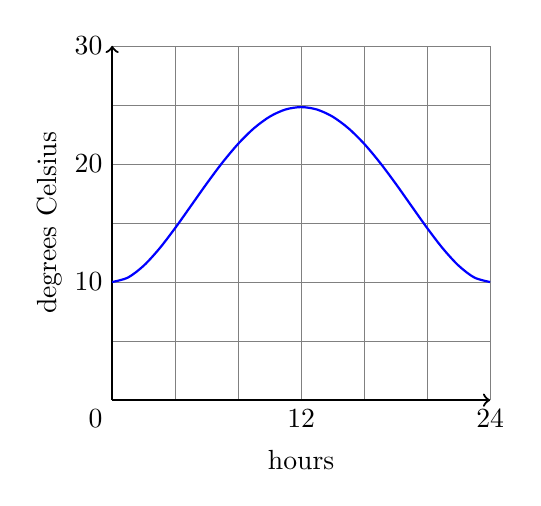
\begin{tikzpicture}
[
	closedpt/.style={circle,draw,fill,inner sep=0pt,minimum size=4pt},
	openpt/.style={circle,draw,inner sep=0pt,minimum size=4pt},
	yscale=0.15,
	xscale=2
]

	% grid
	\foreach \x in {0,0.4,0.8,1.2,1.6,2.0,2.4} {
		\draw[very thin,gray] (\x,\ymin) -- (\x,\ymax);
	}
	\foreach \y in {0,5,10,...,30} {
		\draw[very thin,gray] (\xmin,\y) -- (\xmax,\y);
	}

	% label grid
	\node[below] at (1.2,0) {$12$};
	\node[below] at (2.4,0) {$24$};
	\foreach \y in {10,20,30} {
		\node[left] at (0,\y) {$\y$};
	}
	\node[below left] at (0,0) {$0$};

	% axes
	\draw[->,thick] (\xmin,0) to node[below,yshift=-0.5cm] {hours} (\xmax,0);
	\draw[->,thick] (0,\ymin) to node[rotate=90,yshift=0.8cm] {degrees Celsius} (0,\ymax);

	% graph
	\draw[thick, blue, domain=0:2.4, smooth] plot (\x,{\func});

\end{tikzpicture}
